% !TeX spellcheck = da_DK
\subsection{Påvirkning på encephalon}\label{HjerneSenMot}
Cerebrum er den største region af encephalon og kan deles op i to hjernehalvdele. Her sker en processering af sanserne, tale, tanker, synet, hukommelsen og følelser. \cite{Martini2012} For en yderligere beskrivelse af hjernens anatomi, nervefysiologi samt biologisk kommunikation se bilag \ref{AppNerve}. Som tidligere nævnt i afsnit \ref{IskaemiskApp} er 80-85\% af apopleksitilfældene iskæmiske og rammer hyppigst i media arterien, der forsyner det meste af cerebrum med blod. Derfor er det ofte sensoriske- og motoriske områder, der bliver skadet ved et apopleksitilfælde. \cite{Kruuse2015a,Gade2004,Boss2010} For at opretholde balancen kræves et samarbejde af de sensoriske- og motoriske områder i encephalon som ses på \figref{Enc}.

\begin{figure}[H]
	\centering
	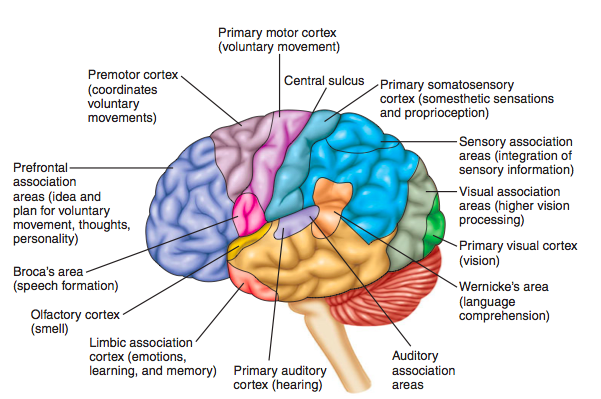
\includegraphics[scale=0.6]{figures/bProblemanalyse/Encephalon2.png}
	\caption{På figuren ses de sensoriske og motoriske regioner på den venstre hjernehalvdel af cerebrum. \textit{(Revideret)} \cite{Stanfield2014}}
	\label{Enc}
\end{figure}

De sensoriske- og motoriske områder har stor indflydelse på hinanden. I \tableref{tabelencephalon} vil områderne i encephalon fremgå, samt deres funktion ift. balancen. Ved apopleksi kan flere områder rammes samtidig, hvilket kan gøre at flere funktioner svækkes. Da balancen er styret af flere forskellige områder i encephalon betyder en skade på f.eks. det visuelle cortex ikke at man mister balancen helt. 

\begin{center}
\begin{table} [H]
  \begin{tabular}{ | l | p{10cm} |}
    \hline
    \textbf{Område i encephalon} & \textbf{Funktioner} \\ \hline
 	Cerebellum & Modtager proprioreceptiv og vestibulær information fra medulla spinalis og truncus encephalius.  Fortolker og koordinerer frivillige bevægelser. \\ \hline
 	Det visuelle cortex & Fortolker lyssignaler og videresender informationer omkring rumlige forhold, bevægelse og koordinerer visuelle og somatosensoriske impulser. \\ \hline
 	Det præmotoriske cortex & Integrerer den sensoriske og motoriske systemer og igangsætter bevægelse som respons på visuelle eller auditive stimuli. \\ \hline
 	Det præfrontale cortex & Koordinerer information fra de andre kortex og udarbejder abstrakte intellektuelle funktioner, som at forudse hvilken effekt en handling vil have. Bearbejdere eksterne sanseindtryk inden der foretages en handling. \\ \hline
 	Truncus Encephalius & Modtager vestibulær information fra det indre ører, som fortæller hovedets placering i rummet og generel balance ift. til tyngdekraften. \\
    \hline
    \end{tabular}
    \caption{På tabellen ses en oversigt over de områder af encephalon, som påvirker balancen, samt deres funktion. Områder kan yderligere ses på \figref{Enc} \cite{Martini2012, Moos2010}}
    \label{tabelencephalon}
\end{table}
\end{center}

De sensoriske- og motoriske nervebaner fra sensorisk- og motorisk cortex løber ned gennem medulla spinalis og leder derved impulser ud til target organer og muskler og tilbage igen. Nervebanerne fra hhv. højre og venstre hjernehalvdel krydser i medulla oblongata eller i medulla spinalis. Denne krydsning betyder, at afferente signaler fra højre side af kroppen behandles i venstre hjernehalvdel, der sender efferente signaler tilbage til højre side af kroppen. \cite{Martini2012,Stanfield2014} Dette medfører, at et apopleksitilfælde i højre hjernehalvdel kan give sensoriske- og motoriske skader i venstre kropsdel og omvendt med venstre hjernehalvdel. \cite{Sundhedsstyrelsen2009,Nichols1997} %Et apopleksitilfælde kan derved lede til neglekt eller problemer med balancen .

Hver muskelgruppe har sine egne dedikerede nerveceller. Antallet af nerveceller til hver muskel afhænger af, hvor præcis legemets bevægelse skal være. Flere nerveceller gør musklens bevægelse mere præcis. \cite{Stanfield2014} Nervecellerne har en bestemt placering i cerebral cortex. Derfor vil et apopleksitilfælde et bestemt sted ramme en bestemt muskel. F.eks. vil en skade på det auditive cortex kunne medføre balanceproblemer, da det derved er svært for patienten at vide hvor hovedet er placeret i rummet. \cite{Mao2014} Efter et apopleksitilfælde har encephalon en naturlig tilpasning ift. at genskabe disse tabte funktioner. I nogle tilfælde kan encephalon genskabe skadede nerver eller finde en anden vej for funktionen, som en eventuelt tabt nerve skulle udføre. \cite{Martini2012} Denne mekanisme kaldes plasticitet \cite{Ramanathan2006}. 

\subsection{Plasticitet}
Encephalon kan ændre eller tilpasse sig de stimuli, den udsættes for, hvilket kaldes encephalons plasticitet eller nerveplasticitet. Processen sker kontinuerligt igennem hele livet, men encephalon kan ikke danne nye nerver. \cite{Stanfield2014} Under et apopleksitilfælde forekommer der iltmangel til encephalon, og nervecellerne kan derved blive skadet eller gå tabt \cite{Schulze2011}. Celledød medfører, at den døde nerve mister sine forbindelser til fungerende nerver. Denne forbindelsesafbrydelse i encephalon bevirker, at der kan opstå en kaskade af mistet kommunikation i de eksisterende nerver. Herved kan en nerves celledød påvirke andre områder af encephalon end blot der, hvor skaden er sket. \cite{Raine2009} Encephalon vil benytte sig af sin plasticitet og omlægge det eksisterende nervenetværk til et nyt. Encephalon vil aktivere nogle signalstoffer, som kan finde en alternativ metode til at gennemføre den ønskede handling. \cite{Rugnett2015}  Som nævnt kan encephalon ikke danne nye nerver efter celledød, hvilket betyder, at der ikke kan generhverves præcis samme funktion som tidligere men evt. en lignende funktion. %Encephalon vil forsøge at kompensere for de tabte nerver ved at danne nye forbindelser og kommunikationsveje, hvilket 
Plasticitet kan deles op i tre fænomener: \cite{Raine2009}

\begin{itemize}
	\item Denervation Supersensitivity er en afbrydelse imellem akson og synapse og medfører, at synapsen bliver overfølsom og derved lettere påvirket til at lave nye synapseforbindelser.
	\item Unmasking of Silent (Latent) Synapses sker når synapser, der har fuld funktionalitet men ingen effekt på slutstedet, afsløres, hvorefter der opstår en aktivitet og effekt. Dvs. synapsen fungerer, men encephalon er ikke opmærksom på dette.
	\item Collateral Sprouting sker hvis to nerver innerverer på samme slutsted, og den ene nerve dør. Så vil den anden nerve spire ind i den skadede nerves telodendron, og funktionen vil derved genvindes.
\end{itemize}

Ud fra disse tre fænomener findes der en fysiologisk baggrund for rehabilitering. Nerveplasticitet er særlig øget op til en måned efter et apopleksitilfælde. Det er derfor vigtigt at foretage genoptræning i denne periode, så encephalon kan danne nye forbindelser og kommunikationsveje. \cite{Rugnett2015} Gentagelser af en færdighed effektiviserer synapseforbindelser, hvilket betyder, at den kompenserende færdighed styrkes. \cite{Stanfield2014}. Den kompenserende færdighed dækker over de kompenserende bevægelser som kroppen skaber for at erstatte en tabt funktionsevne \cite{Takeuchi2012,Leea2009}. %Udover plasticitet vil kroppen også skabe såkaldte kompenserende bevægelser for at erstatte en tabt funktionsevne. %Kompensatoriske bevægelser er et resultat af, at kroppen stadigvæk har brug for en givet funktion, men pga. tabt sensorisk og motorisk funktion ikke kan udføre bevægelsen. Disse kompenserende bevægelsesmønstre kan medføre et funktionelt dårligt resultat og kan være associeret med langsigtede konsekvenser såsom smerte og reduceret funktionsevne \cite{Takeuchi2012,Leea2009}.


%\subsection{Plasticitet}
%Encephalon kan ændre eller tilpasse sig de stimuli, den udsættes for, hvilket kaldes encephalons plasticitet eller nerveplasticitet. Dette sker kontinuerligt igennem hele livet, men encephalon kan ikke danne nye nerver. \cite{Stanfield2014} Under et apopleksitilfælde forekommer der iltmangel til encephalon, og nervecellerne kan derved blive skadet eller gå tabt. \cite{Schulze2011} Denne celledød gør, at den døde nerve mister sine forbindelser til raske nerver. Denne forbindelsesafbrydelse i encephalon bevirker, at der kan opstå en kaskade af mistet kommunikation i de eksisterende nerver. Herved kan en nerves celledød altså påvirke andre områder af encephalon end blot der, hvor skaden er sket. \cite{Raine2009} Encephalon vil benytte sig af sin plasticitet og omlægge det eksisterende nervenetværk. Encephalon vil aktivere nogle signalstoffer, som kan finde en alternativ metode til at gennemføre den ønskede handling. \cite{Rugnett2015}  Som sagt kan encephalon ikke danne nye nerver efter celledød, hvilket betyder, at der ikke kan generhverves præcis samme funktion som tidligere men evt. en lignende funktion. Men encephalon vil forsøge at kompensere for de tabte nerver ved at danne nye forbindelser og kommunikationsveje, hvilket kan deles op i tre fænomener: \cite{Raine2009}

%\begin{itemize}
	%\item En afbrydelse imellem akson og synapse medfører, at synapsen bliver overfølsom og derved lettere påvirket til at lave nye synapseforbindelser. Dette fænomen kaldes “Denervation Supersensitivity”.
%	\item Synapser, der har fuld funktionalitet men ingen effekt på slutstedet, “afsløres”, hvorefter der opstår en aktivitet og effekt. Dette kaldes “Unmasking of Silent (Latent) Synapses”.
%	\item Hvis to nerver innerverer på samme slutsted, og den ene nerve dør, så vil den anden nerve spire ind i den skadede nerves telodendron, og funktionen vil derved genvindes. Dette kaldes “Collateral Sprouting”.
%>>>>>>> origin/master
%\end{itemize}

%det forrige
%\subsection{Påvirkning på encephalon}\label{HjerneSenMot}

%Cerebrum er den største region af encephalon og kan deles op i to hjernehalvdele. Her sker en processering af sanserne, tale, tanker, synet, hukommelsen og følelser. \cite{Martini2012} For en yderligere beskrivelse af hjernen, nervefysiologi samt biologisk kommunikation se bilag \ref{AppNerve}. De forskellige sensoriske- og motoriske regioner kan ses på \figref{Enc}. Som tidligere nævnt i afsnit \ref{IskaemiskApp} er 80-85\% af apopleksitilfældene iskæmiske og rammer hyppigst i media arterien, der forsyner det meste af cerebrum med blod. Derfor er det ofte sensoriske- og motoriske områder, som bliver skadet ved et apopleksitilfælde. \cite{Sundhed.dk,Gade2004,Boss2010} \\

%\begin{figure}[H]
%	\centering
%	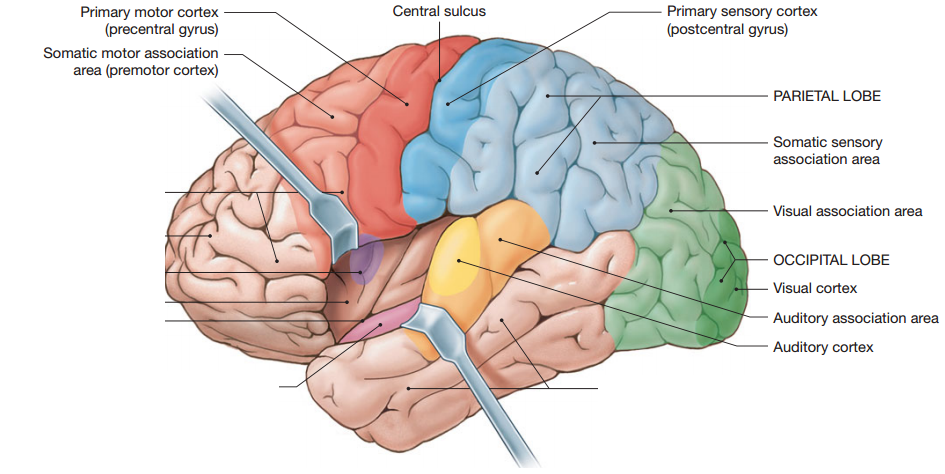
\includegraphics[scale=0.6]{figures/bProblemanalyse/Encephalon.png}
%	\caption{På figuren ses de sensoriske og motoriske regioner på den venstre hjernehalvdel af cerebrum. %\textit{(Revideret)} \cite{Martini2012}}
%	\label{Enc}
%\end{figure}

%De sensoriske- og motoriske nervebaner fra sensorisk- og motorisk cortex løber ned gennem medulla spinalis og leder derved impulser ud til target organer og muskler og tilbage igen. Nervebanerne fra hhv. højre og venstre hjernehalvdel krydser i medulla oblongata eller i medulla spinalis. Denne krydsning betyder, at afferente signaler fra højre side af kroppen behandles i venstre hjernehalvdel, der sender efferente signaler tilbage til højre side af kroppen. \cite{Martini2012,Stanfield2014} Dette medfører, at et apopleksitilfælde i højre hjernehalvdel kan give sensoriske- og motoriske skader i venstre kropsdel og omvendt med venstre hjernehalvdel. \cite{Sundhedsstyrelsen2009,Nichols1997} %Et apopleksitilfælde kan derved lede til neglekt eller problemer med balancen .

%Hver muskelgruppe har sine egne dedikerede nerveceller. Antallet af nerveceller til hver muskel afhænger af, hvor præcis legemets bevægelse skal være. Flere nerveceller gør musklens bevægelse mere præcis. \cite{Stanfield2014} Nervecellerne har en bestemt placering i cerebral cortex. Derfor vil et apopleksitilfælde et bestemt sted ramme en bestemt muskel. F.eks. vil en skade på det auditive cortex kunne medføre balanceproblemer, da det derved er svært for patienten at vide hvor hovedet er placeret i rummet. \cite{Mao2014} 
%\begin{center}
%\begin{tabular}{ | l | p{8cm} |}
%\hline
%Auditive cortex & hej med dig \\ \hline
%\end{tabular}
%\end{table}

%\subsection{Encephalons påvirkning på balance}
%For at opretholde balancen kræves der samarbejde af flere områder af encephalon. Disse har en stor indflydelse på hinanden. Områderne kan ses i \tableref{tabelencephalon}. Ved apopleksi kan flere områder rammes samtidig, hvilket kan gøre at flere funktioner svækkes. Da balancen er styret af flere forskellige områder i encephalon betyder en skade på eksempelvis det visuelle cortex ikke at man mister balancen helt. 

%\begin{center}
%\begin{table} [H]
  %\begin{tabular}{ | l | p{8cm} |}
   % \hline
  %  \textbf{Område i encephalon} & \textbf{Funktioner} \\ \hline
 %	Cerebellum & Modtager proprioreceptiv og vestibulær information fra medulla spinalis og truncus encephalius.  %Fortolker og koordinerer frivillige bevægelser. \\ \hline
 %	Det visuelle cortex & Fortolker lyssignaler og videresender informationer omkring rumlige forhold, bevægelse og %koordinerer visuelle og somatosensoriske impulser. \\ \hline
 %	Det præmotoriske cortex & Integrerer den sensoriske og motoriske systemer og igangsætter bevægelse som respons på %visuelle eller auditive stimuli. \\ \hline
 %	Det præfrontale cortex & Koordinerer information fra de andre kortex og udarbejder abstrakte intellektuelle %funktioner, som at forudse hvilken effekt en handling vil have. Bearbejdere eksterne sanseindtryk inden der foretages %en handling. \\ \hline
 %	Truncus Encephalius & Modtager vestibulær information fra det indre ører, som fortæller hovedets placering i %rummet og generel balance ift. til tyngdekraften. \\
    %\hline
   % \end{tabular}
 %   \caption{Tabel over de områder af encephalon som påvirker balancen, samt deres funktion. \cite{Martini2012, %Moos2010}}
 %   \label{tabelencephalon}
%\end{table}
%\end{center}


%Encephalon har en naturlig tilpasning. Dette medfører, at den i nogle tilfælde kan genskabe skadede nerver eller finde en anden vej for funktionen, som en eventuelt tabt nerve skulle udføre. \cite{Martini2012} Denne mekanisme kaldes plasticitet \cite{Ramanathan2006}.